%%%%%%%%%%%%%%%%%%%%%%%%%%%%%%%%%%%%%%%%%
% Jacobs Portrait Poster
% LaTeX Template
% Version 1.0 (31/08/2015)
% (Based on Version 1.0 (29/03/13) of the landscape template
%
% Created by:
% Computational Physics and Biophysics Group, Jacobs University
% https://teamwork.jacobs-university.de:8443/confluence/display/CoPandBiG/LaTeX+Poster
% 
% Further modified by:
% Nathaniel Johnston (nathaniel@njohnston.ca)
%
% Portrait version by:
% John Hammersley
%
% The landscape version of this template was downloaded from:
% http://www.LaTeXTemplates.com
%
% License:
% CC BY-NC-SA 3.0 (http://creativecommons.org/licenses/by-nc-sa/3.0/)
%
%%%%%%%%%%%%%%%%%%%%%%%%%%%%%%%%%%%%%%%%%

%----------------------------------------------------------------------------------------
%	PACKAGES AND OTHER DOCUMENT CONFIGURATIONS
%----------------------------------------------------------------------------------------

\documentclass[final]{beamer}

\usepackage[scale=1.24]{beamerposter} % Use the beamerposter package for laying out the poster
\usetheme{confposter} % Use the confposter theme supplied with this template
\usepackage{booktabs}
\usepackage{colortbl} % Required to have colors for table rows
\usepackage{graphicx}  % Required for including images
\usepackage{subcaption}



\setbeamercolor{block title}{fg=ngreen,bg=white} % Colors of the block titles
\setbeamercolor{block body}{fg=black,bg=white} % Colors of the body of blocks
\setbeamercolor{block alerted title}{fg=white,bg=dblue!70} % Colors of the highlighted block titles
\setbeamercolor{block alerted body}{fg=black,bg=dblue!10} % Colors of the body of highlighted blocks
% Many more colors are available for use in beamerthemeconfposter.sty

%-----------------------------------------------------------
% Define the column widths and overall poster size
% To set effective sepwid, onecolwid and twocolwid values, first choose how many columns you want and how much separation you want between columns
% In this template, the separation width chosen is 0.024 of the paper width and a 4-column layout
% onecolwid should therefore be (1-(# of columns+1)*sepwid)/# of columns e.g. (1-(4+1)*0.024)/4 = 0.22
% Set twocolwid to be (2*onecolwid)+sepwid = 0.464
% Set threecolwid to be (3*onecolwid)+2*sepwid = 0.708

\newlength{\sepwid}
\newlength{\onecolwid}
\newlength{\twocolwid}
\newlength{\threecolwid}
\setlength{\paperwidth}{33.1in} % A0 width: 46.8in
\setlength{\paperheight}{46.8in} % A0 height: 33.1in
\setlength{\sepwid}{0.025\paperwidth} % Separation width (white space) between columns
\setlength{\onecolwid}{0.30\paperwidth} % Width of one column
\setlength{\twocolwid}{0.464\paperwidth} % Width of two columns
\setlength{\threecolwid}{0.708\paperwidth} % Width of three columns
\setlength{\topmargin}{-0.5in} % Reduce the top margin size
%-----------------------------------------------------------

\graphicspath{{./figures/}}

% If your conference documentclass or package defines these macros,
% change these macros to different names.
\newcommand*{\affaddr}[1]{#1} % No op here. Customize it for different styles.
\newcommand*{\affmark}[1][*]{\textsuperscript{#1}}

% Data colors
\definecolor{CBOne}{HTML}{a6cee3}
\definecolor{CBTwo}{HTML}{1f78b4}
\definecolor{CBThree}{HTML}{b2df8a}
\definecolor{CBFour}{HTML}{33a02c}



%----------------------------------------------------------------------------------------
%	TITLE SECTION 
%----------------------------------------------------------------------------------------

\title{Block-distributed Gradient Boosted Trees} % Poster title

\author{Theodore Vasiloudis\affmark[1], Hyunsu Cho\affmark[2], Henrik Bostr\"{o}m\affmark[3]} % Author(s)

\institute{\affmark[1]\,Research Institutes of Sweden, \affmark[2]\,Amazon Web Services, \affmark[3]\,KTH Royal Institute of Technology.} % Institution(s)
% TODO Improve the author symbols
%----------------------------------------------------------------------------------------

\begin{document}

\addtobeamertemplate{block end}{}{\vspace*{2ex}} % White space under blocks
\addtobeamertemplate{block alerted end}{}{\vspace*{2ex}} % White space under highlighted (alert) blocks

\setlength{\belowcaptionskip}{2ex} % White space under figures
\setlength\belowdisplayshortskip{2ex} % White space under equations

\begin{frame}[t] % The whole poster is enclosed in one beamer frame

\begin{columns}[t] % The whole poster consists of three major columns, the second of which is split into two columns twice - the [t] option aligns each column's content to the top

\begin{column}{\sepwid}\end{column} % Empty spacer column

\begin{column}{\onecolwid} % The first column

	%----------------------------------------------------------------------------------------
	%	SUMMARY
	%----------------------------------------------------------------------------------------
	
	\begin{alertblock}{Summary}
	% TODO Maybe want to left align this
	We introduce block-distributed training for 
	gradient boosted trees (GBT), enhancing their
	scalability.
	
	\noindent
	Our contributions are the following:
	
	\begin{itemize}
	\item The first algorithm for data \emph{and} feature parallel training of GBTs.
	\item Adapt the Quickscorer fast prediction algorithm to the
		block distributed setting.
	\item We achieve orders of magnitude improved communication cost
		by taking advantage of data sparsity.
	\end{itemize}
	
	\end{alertblock}
	
	%----------------------------------------------------------------------------------------
	%	INTRODUCTION
	%----------------------------------------------------------------------------------------
	
	\begin{block}{Introduction}
	
		\textbf{Gradient Boosted Trees}: One of the most widely used algorithms
		in machine learning, including IR tasks like learning-to-rank
		and CTR prediction.
	
		\vspace{15pt}
		\textbf{Why it's important:}
	
		\begin{itemize}
			\item We need highly scalable algorithms for enterprise scale, \emph{high-dimensional
			data}.
			\item Training on such data is done in clusters, where network communication
			is the \emph. %TODO Is this why it's important or a problem of SOTA?
			% Alternative With billions of data points and features, we need to take full advantage of the ...
		\end{itemize}
	
		\textbf{Why it's difficult:}
	
		\begin{itemize}
	
		\item All current distributed GBT algorithms \emph{only use row distribution},
			and for feature parallel training, assume \emph{all data fit into the memory} of each worker.
		\item In the block-distributed setting \emph{no worker has a full view} of any data point.
			This presents additional challenges for training and prediction.
		\end{itemize}
	
	\end{block}

%------------------------------------------------

	\begin{block}{Gradient Boosted Trees}
	
		\begin{figure}
		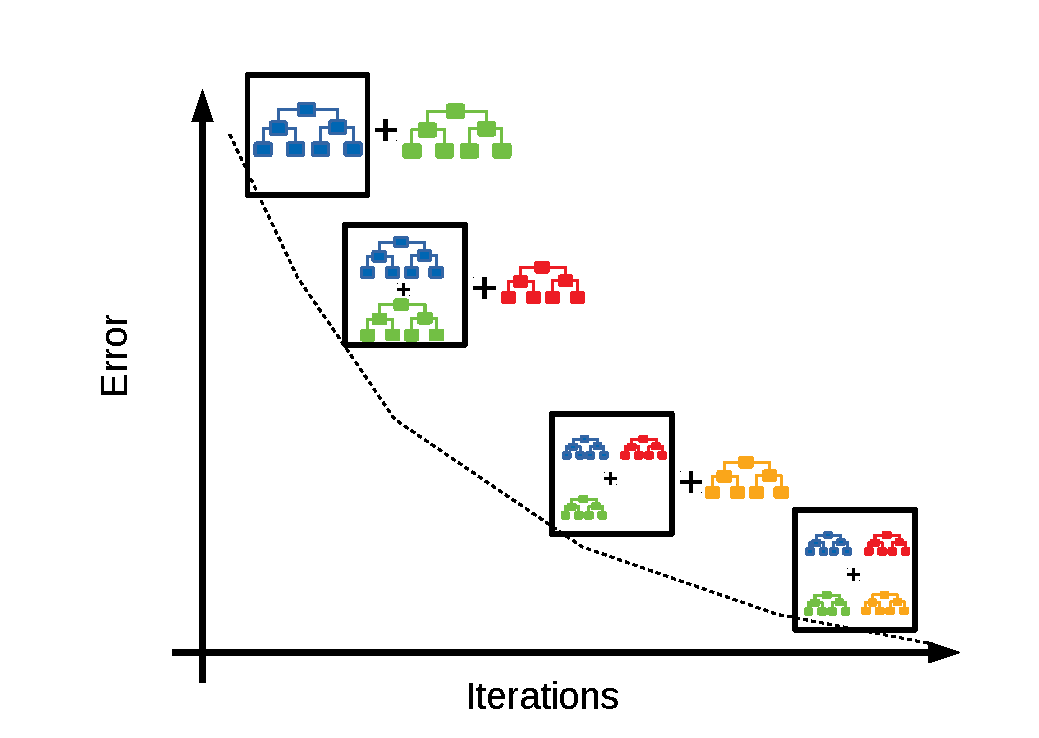
\includegraphics[width=\onecolwid]{gbt-illustration}
			\label{fig:gbt-training}
		\end{figure}
	
	\end{block}



%----------------------------------------------------------------------------------------

\end{column} % End of the first column

\begin{column}{\sepwid}\end{column} % Empty spacer column

\begin{column}{\onecolwid} % Begin second column
	
	\begin{block}{Block-distributed data}
		\begin{figure}
			\centering
			\begin{subfigure}[t]{0.45\onecolwid}
				\centering
				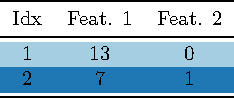
\includegraphics[height=4cm]{w1}
				\caption{Worker 1.}
			\end{subfigure}
			\quad
			\begin{subfigure}[t]{0.45\onecolwid}
				\centering
				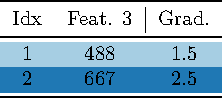
\includegraphics[height=4cm]{w2}
				\caption{Worker 2.}
			\end{subfigure}
			\\
			\vspace{15pt}
			\begin{subfigure}[t]{0.45\onecolwid}
			\centering
			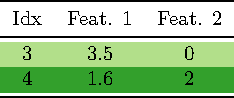
\includegraphics[height=4cm]{w3}
			\caption{Worker 3.}
			\end{subfigure}
			~
			\begin{subfigure}[t]{0.45\onecolwid}
				\centering
				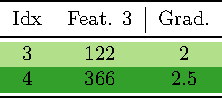
\includegraphics[height=4cm]{w4}
				\caption{Worker 4.}
			\end{subfigure}
		
%			\caption{Local gradient histograms for row-distributed data. Note the existence of multiple
%				zero values that would nonetheless need to be communicated using a dense communication pattern like
%				MPI allreduce.}
			\label{fig:grad-row-dist}
		\end{figure}
		

	\end{block}
	
	
	\begin{block}{Block-distributed Quickscorer}
		
		In the block-distributed setting, prediction requires communication.
		To minimize the size of the data being communicated we develop
		a block-distributed version of the Quickscorer algorithm.
		
		\begin{figure}
			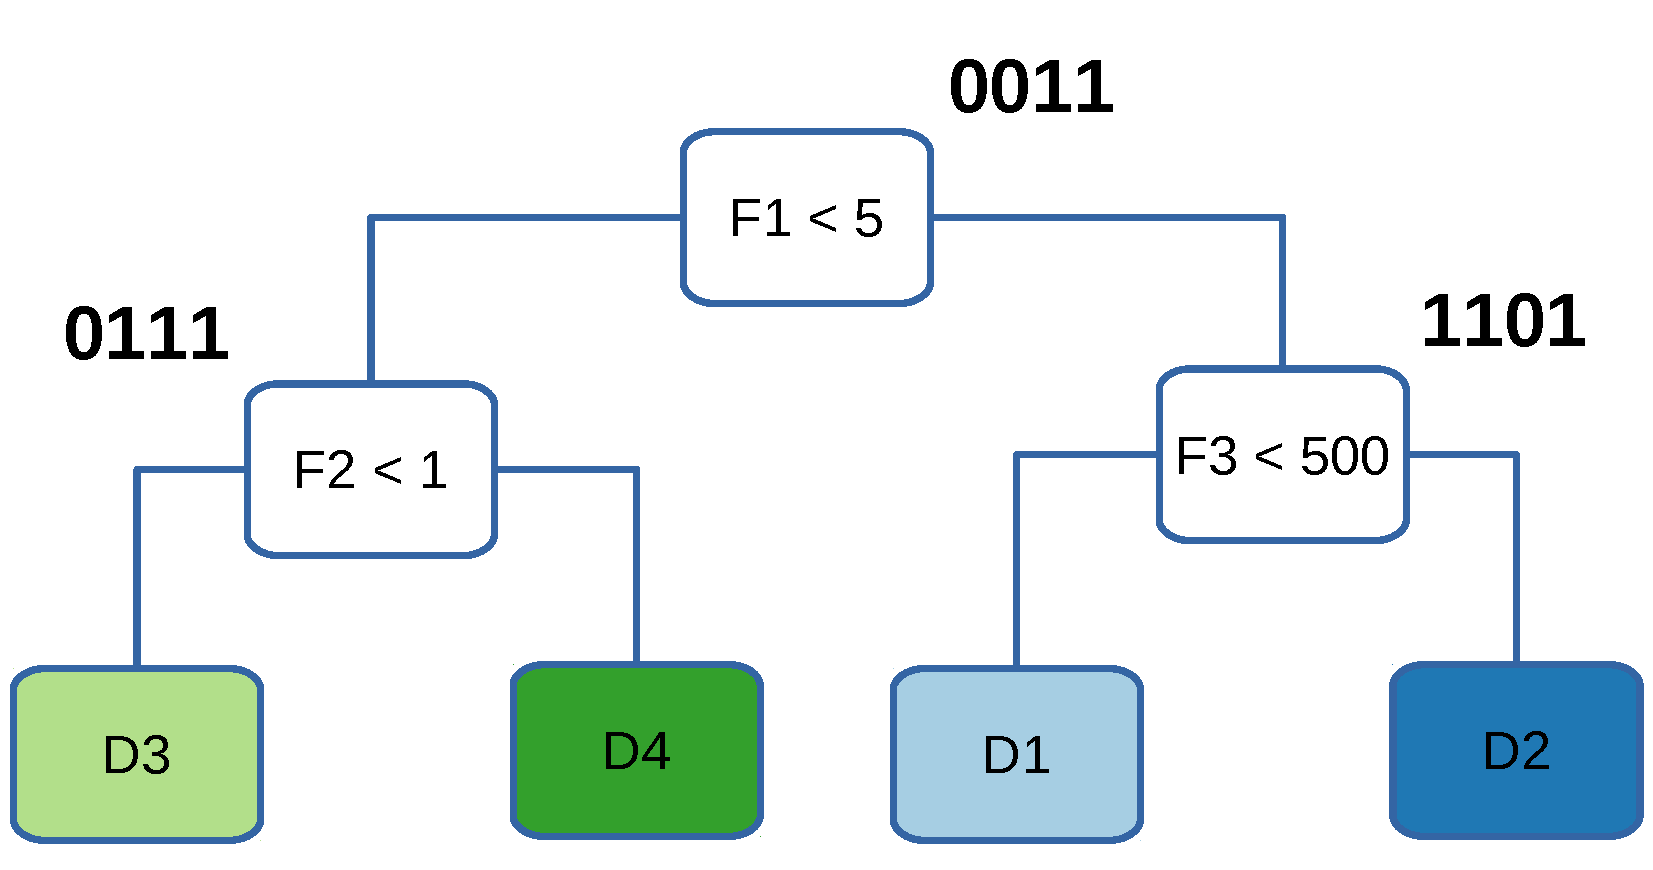
\includegraphics[width=\onecolwid]{decision_tree_bitstrings}
%			\caption{Quickscorer example.}
			\label{fig:quickscorer}
		\end{figure}
		
	\end{block}
	
	\begin{block}{Gradient Histograms}
		
		\begin{itemize}
			\item The most computationally intensive part of GBT training is gradient
			histogram calculation.
			
			\item These assign the gradients to specific ranges of values for each
			feature (buckets).
			
			\item We use them to calculate the potential gain from splitting at particular
			feature value.
		\end{itemize}
		
		\begin{figure}
			% TODO: Increase text sizes in the data
			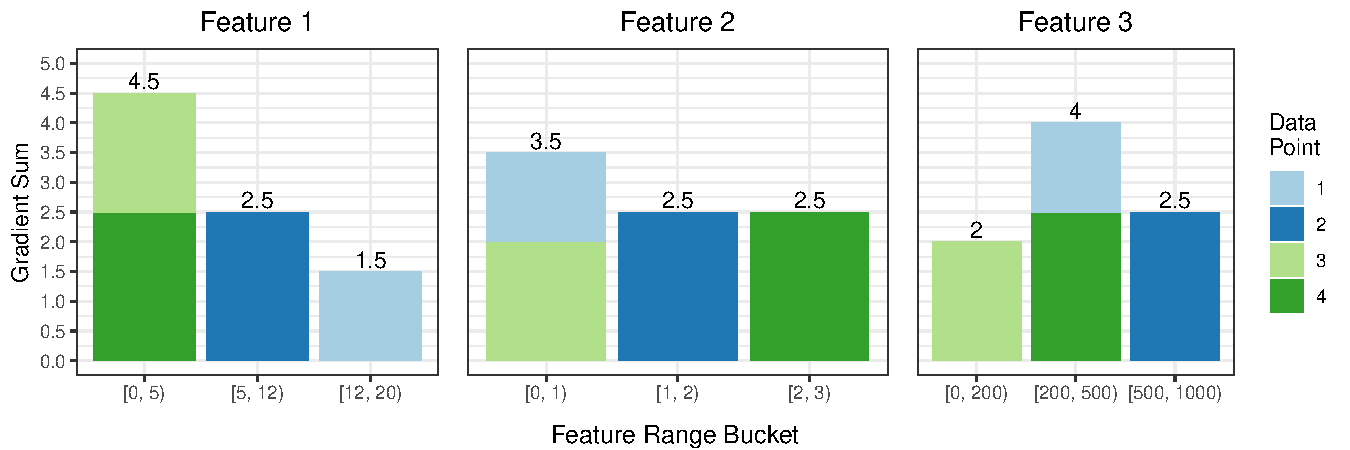
\includegraphics[width=\onecolwid]{all-features-grad}
			\label{fig:grad-features}
		\end{figure}
		
	\end{block}

	\begin{block}{Gradient Histograms are sparse}
		\begin{figure}
			\centering
			\begin{subfigure}[t]{\textwidth}
				\centering
				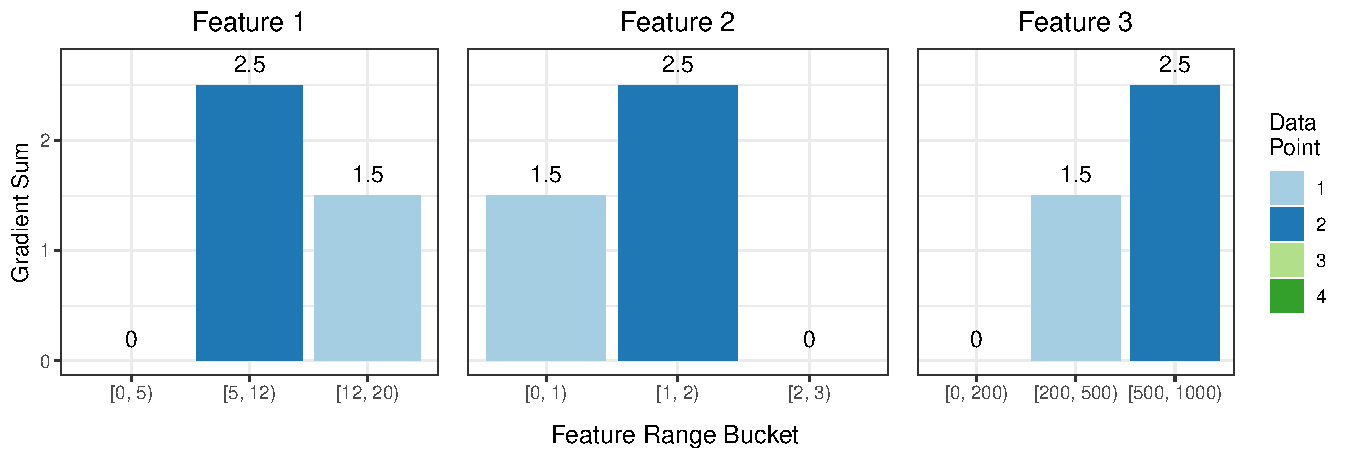
\includegraphics[width=\linewidth]{all-features-grad-rowdist-w1}
				\caption{Local gradient histogram for Worker 1.}
				\label{fig:grad-row-dist-w1}
			\end{subfigure}
			\\
			\begin{subfigure}[t]{\textwidth}
				\centering
				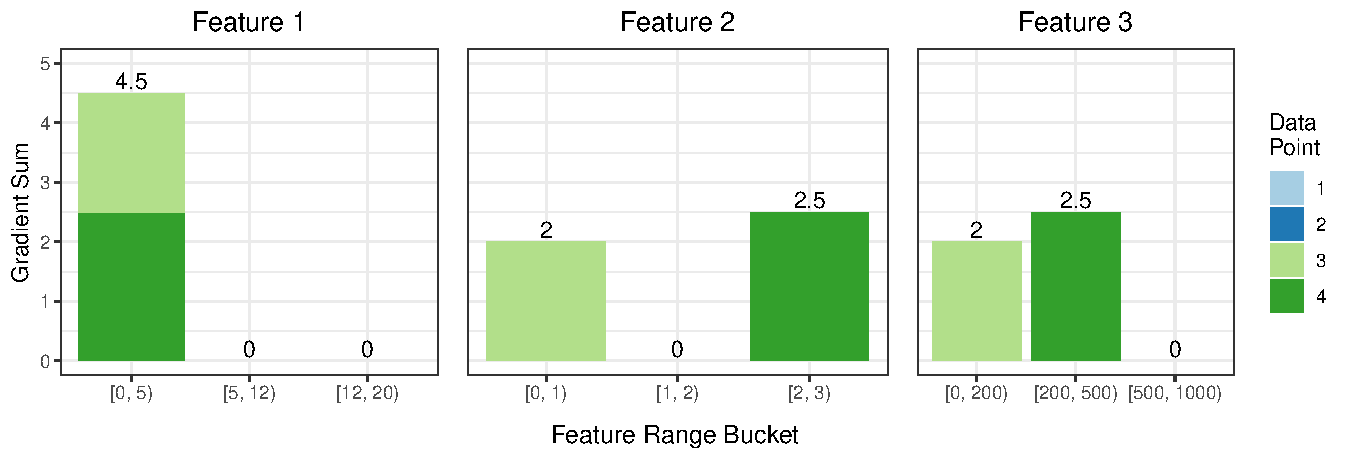
\includegraphics[width=\linewidth]{all-features-grad-rowdist-w2}
				\caption{Local gradient histogram for Worker 2.}
				\label{fig:grad-row-dist-w2}
			\end{subfigure}
%			\caption{Local gradient histograms for row-distributed data. Note the existence of multiple
%				zero values that would nonetheless need to be communicated using a dense communication pattern like
%				MPI allreduce.}
%			\label{fig:grad-row-dist}
		\end{figure}
		% TODO: Trim spacing between blocks
	\end{block}

	
\end{column} % End of the second column

\begin{column}{\sepwid}\end{column} % Empty spacer column

\begin{column}{\onecolwid} % The third column
	
	\begin{block}{Sparse communication}
		
		We create sparse matrices for the histograms, and communicate
		those, using the Parameter Server.
		
		\begin{equation*}
			\begin{pmatrix}
			0 & 0 & 0 & 0 \\
			5 & 8 & 0 & 0 \\
			0 & 0 & 3 & 0 \\
			0 & 6 & 0 & 0
			\end{pmatrix} \equiv 
			\begin{aligned}
			A &= [5, 8, 3, 6] \\
			IA &= [0, 0, 2, 3, 4] \\
			JA &= [0, 1, 2, 1]
			\end{aligned}
		\end{equation*}
		
		Using a sparse format we can significantly shrink the number of values being communicated.
	
	\end{block}
	
	\begin{block}{Results}

	\begin{figure}
		\centering
		\begin{subfigure}[t]{\textwidth}
			\centering
			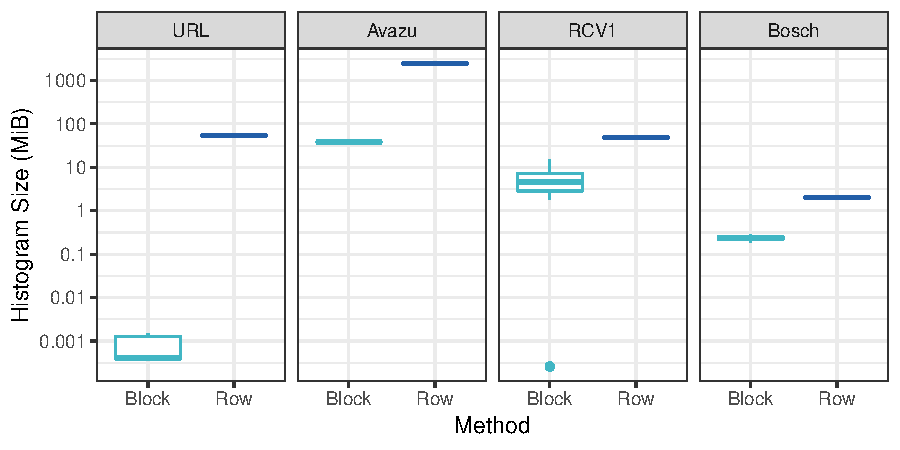
\includegraphics[width=\linewidth]{block-gbt-hist-box}
			\caption{Byte size of histograms being communicated for block (left) and row (right) distributed
				approach.}
		\end{subfigure}
		\\
		\vspace{15pt}
		\begin{subfigure}[t]{\textwidth}
			\centering
			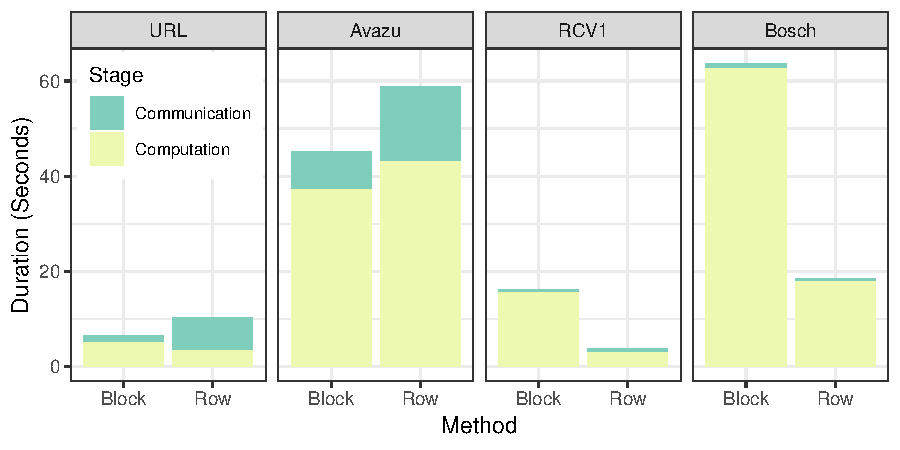
\includegraphics[width=\linewidth]{block-gbt-time}
			\caption{Time for histogram creation, including computation and
				communication.}
		\end{subfigure}
	\end{figure}

	\end{block}



	%----------------------------------------------------------------------------------------
	%	CONCLUSION
	%----------------------------------------------------------------------------------------
	
	\begin{block}{Conclusions}
	
		\begin{itemize}
			\item We developed the first algorithm for block-distributed GBT training.
			\item Our approach allows for several orders of magnitude improvement in
				communication costs for highly sparse data.
			\item More work needs to be done for dense data to offset the computational
				overhead of the sparse data structures.
		\end{itemize}
		
	\end{block}
	
	
	%----------------------------------------------------------------------------------------
	%	REFERENCES
	%----------------------------------------------------------------------------------------
	
	%\begin{block}{References}
	%
	%\nocite{*} % Insert publications even if they are not cited in the poster
	%\small{\bibliographystyle{unsrt}
	%\bibliography{sample}\vspace{0.75in}}
	%
	%\end{block}
	
	%----------------------------------------------------------------------------------------
	%	ACKNOWLEDGEMENTS
	%----------------------------------------------------------------------------------------
	
	\setbeamercolor{block title}{fg=red,bg=white} % Change the block title color
	
	\begin{block}{Acknowledgments}
	
	\small{\rmfamily{This work was performed in part while Theodore was
			completing an internship at Amazon Web Services. Additional funding for Theodore was provided by the
		Swedish Foundation for Strategic Research, grant BD15-0006.}} \\
	
	\end{block}
	
	%----------------------------------------------------------------------------------------
	%	CONTACT INFORMATION
	%----------------------------------------------------------------------------------------
	
	\setbeamercolor{block alerted title}{fg=black,bg=norange} % Change the alert block title colors
	\setbeamercolor{block alerted body}{fg=black,bg=white} % Change the alert block body colors
	
	\begin{alertblock}{Contact}
	
	\begin{itemize}
	\item Email: \href{mailto:tvas@kth.se}{tvas@kth.se}
	\item Twitter: \href{https://www.twitter.com/thvasilo}{@thvasilo}
	\end{itemize}
	
	\end{alertblock}
	
	\begin{center}
	\begin{tabular}{ccc}
	
\includegraphics[height=2cm]{rise_logo_horizontal_cmyk.pdf} \hfill & 
	
\includegraphics[height=2cm]{amazon} \hfill & 
\includegraphics[height=3cm]{kth}
	\end{tabular}
	\end{center}

%----------------------------------------------------------------------------------------

\end{column} % End of the fourth column

\begin{column}{\sepwid}\end{column} % Empty spacer column

\end{columns} % End of all the columns in the poster

\end{frame} % End of the enclosing frame

\end{document}
